\section{Введение}

Осциллограф является одним из важнейших исследовательских приборов. Чаще всего он применяется для наблюдения и исследования переменных во времени электрических сигналов.

\subsection{Решаемые задачи}

\begin{enumerate}
    \item Исследовать чувствительность пластин вертикального и горизонтального отклонений осциллографической трубки.
    \item Наблюдать с помощью осциллографа синусоидальное напряжение, полученное с выхода генератора.
    \item Получить фигуры Лиссажу и определить частоту исследуемого напряжения по фигурам Лиссажу.
\end{enumerate}

\section{Основная часть}

\subsection{Теоретическая часть}

\subsubsection{Электронно-лучевая трубка}

Электронно-лучевая трубка (рис.~\ref{fig:Scheme1}) — основной элемент осциллографа, состоящий из :
\begin{itemize}
\item Электронной пушки (анод, катод, фокусирующий электрод, нагреватель катода);
\item Отклоняющих пластин (горизонтальных $C_1$ и вертикальных $C_2$);
\item Экрана.
\end{itemize}

\begin{figure}[H]
\centering
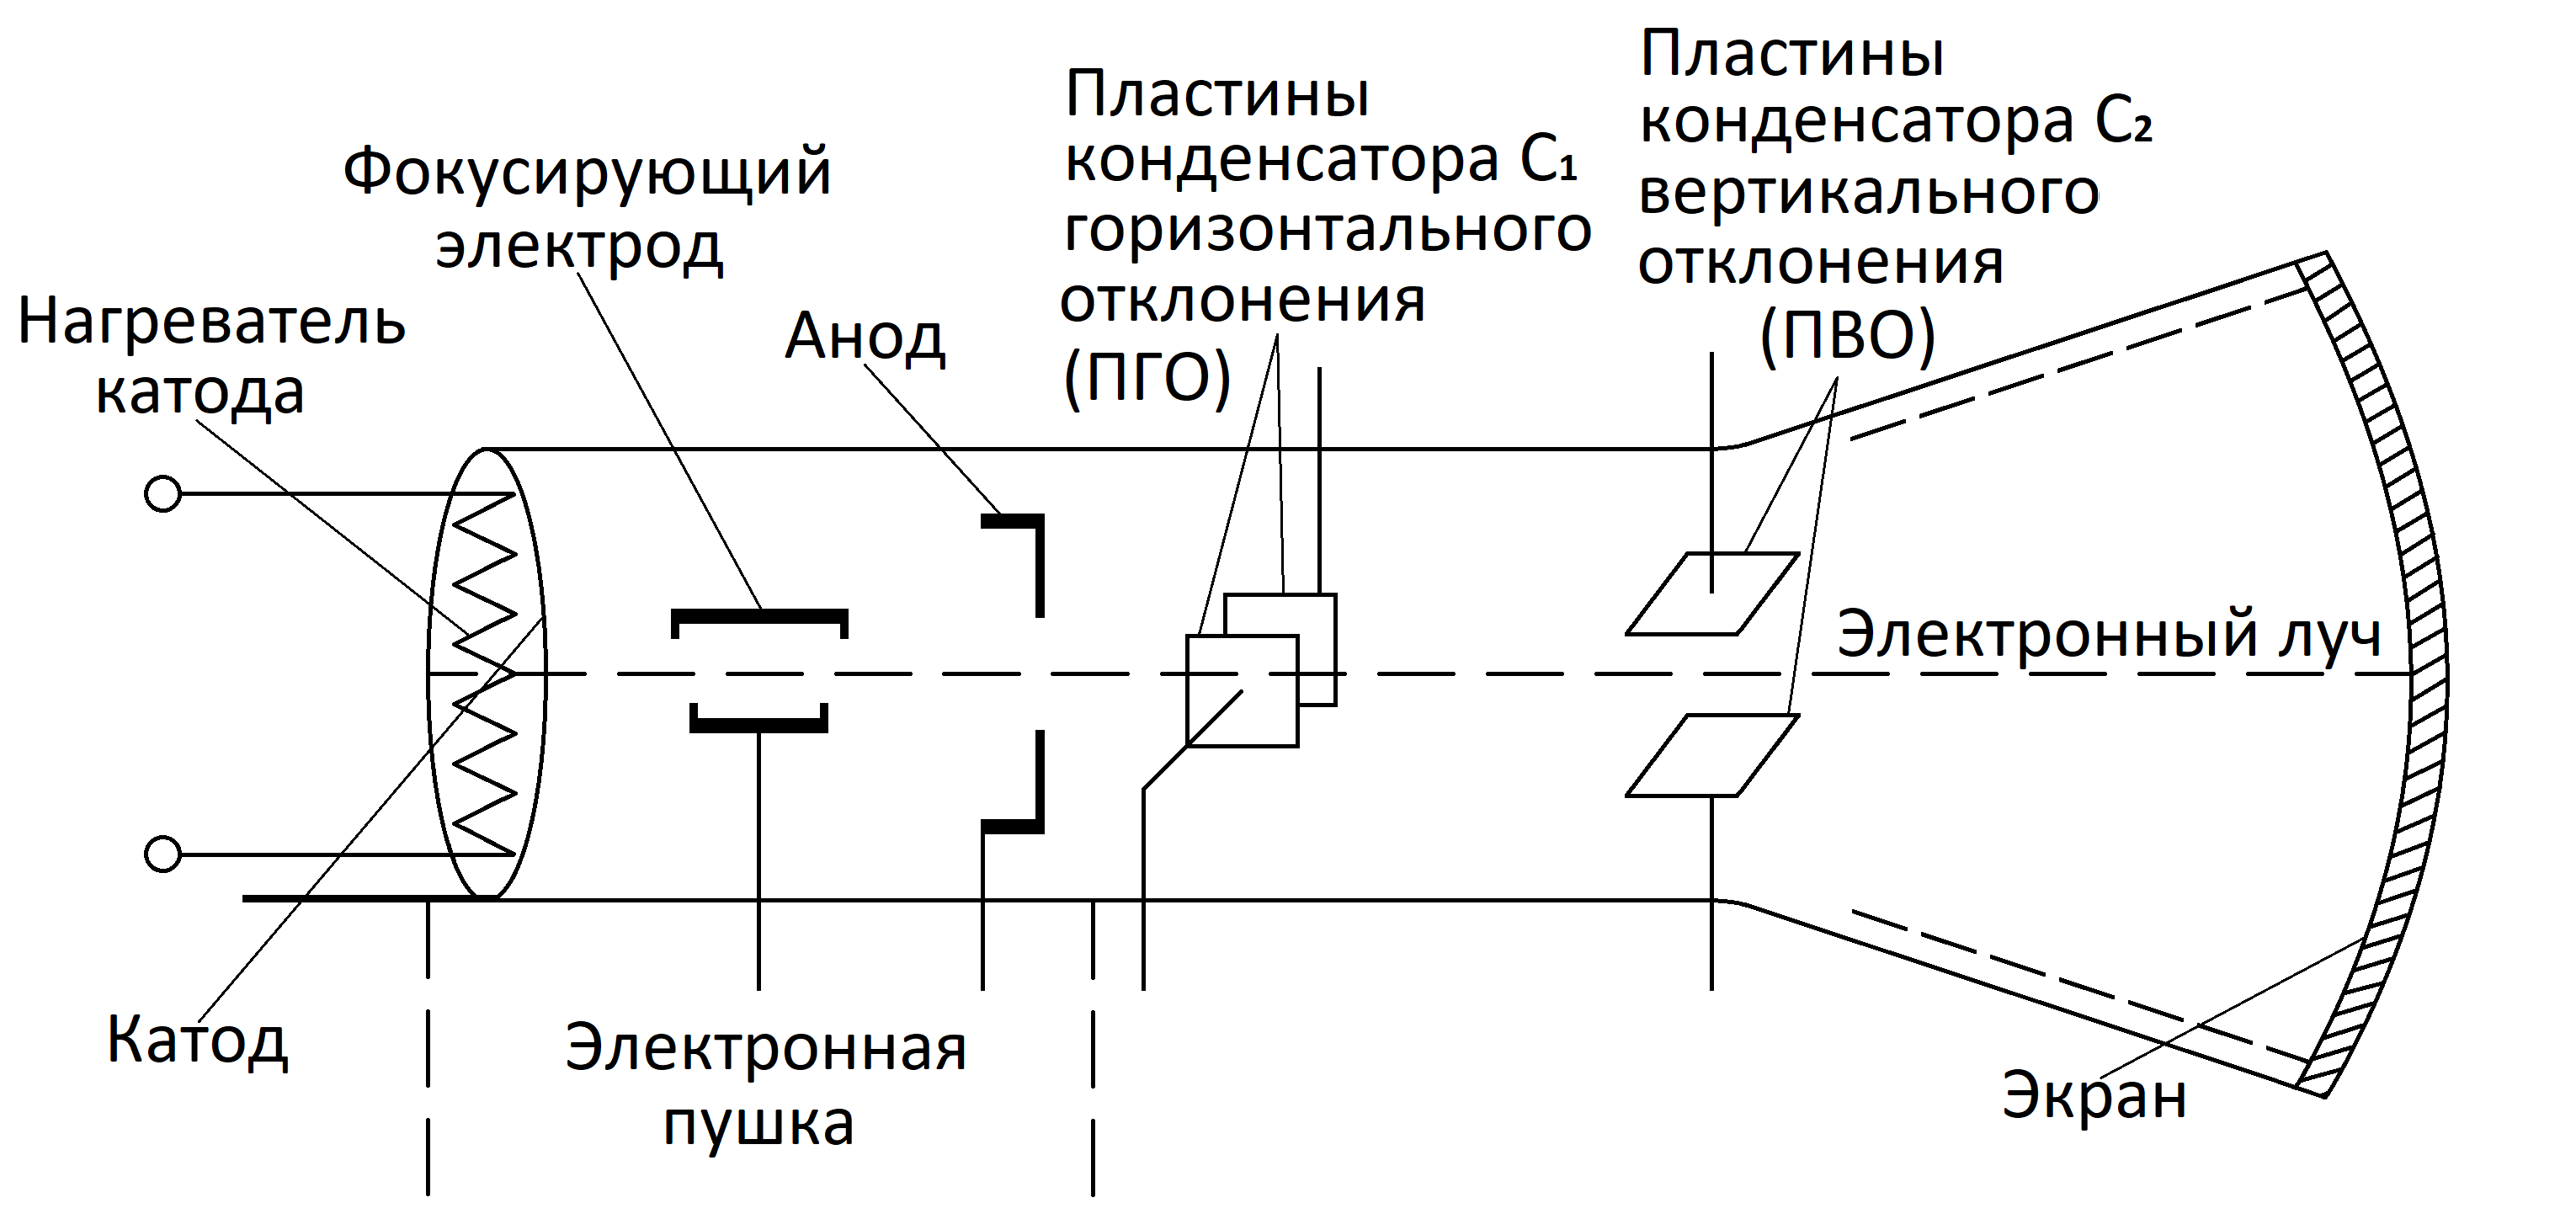
\includegraphics[width=0.8\textwidth]{Scheme1.png}
\caption{Схема электронно-лучевой трубки}
\label{fig:Scheme1}
\end{figure}

Электронно-лучевая трубка — это вакуумный прибор, который преобразует электрические сигналы в видимое изображение. Работа трубки происходит следующим образом:
\begin{enumerate}

\item Формирование электронного луча
\begin{itemize}
\item Катод нагревается нитью накала и испускает электроны (термоэлектронная эмиссия);
\item Фокусирующий электрод сужает электронный поток в узкий луч;
\item Анод ускоряет электроны высоким напряжением.
\end{itemize}

\item Отклонение луча

Луч проходит между двумя парами отклоняющих пластин (Горизонтальные пластины ($C_1$) смещают луч по оси $X$, а вертикальные пластины ($C_2$) — по оси $Y$). Напряжение на пластинах создаёт электрическое поле, отклоняющее электроны пропорционально его величине.
\item Формирование изображения

Электроны попадают на люминофорное покрытие экрана, вызывая свечение в этой точке. При подаче переменного напряжения луч рисует траекторию. Пилообразное напряжение на горизонтальных пластинах создаёт развёртку (луч движется слева направо, затем резко возвращается).
\end{enumerate}

Чувствительность пластин вертикального отклонения высчитывается по формуле:

\begin{equation}
\label{eq:1}
   S_y = \frac{L_{(+-)}}{U_{(+-)}} \left( \frac{\text{мм}}{\text{В}} \right)
\end{equation}

где $L_{(+-)}$ — смещение пятна, $U_{(+-)}$ — приложенное напряжение. При подаче переменного синусоидального напряжения $u = U_0cos(2{\pi}ft + \varphi_0)$ чувствительность пластин определяется по формуле:

\begin{equation}
\label{eq:2}
   S_y = \frac{L_{\sim}}{2\sqrt{2}U_{\text{eff}}} \simeq 0,354 \frac{L_{\sim}}{U_{\text{eff}}}
\end{equation}

где $L_{\sim}$ — длина светящейся линии (двойная амплитуда приложенного напряжения) $U_{\text{eff}} = \frac{U_0}{\sqrt2}$ — эффективное значение синусоидального напряжения.

При подаче разных синусоидальных сигналов на вертикальные и горизонтальные пластины луч начинает двигаться по сложной траектории, описываемой уравнениями: $U_x = (U_0)_xcos(2{\pi}f_x + \varphi_x)$ и $U_y = (U_0)_ycos(2{\pi}f_y + \varphi_y)$. В зависимости от соотношения частот $f_x$ и $f_y$ и фаз $\varphi_x$ и $\varphi_y$ на экране возникают различные изображения. В случае, описываемом уравнением:

\begin{equation}
\label{eq:3}
   f_x = nf_y
\end{equation}

где $n = 1, 2, \frac{1}{2}, \frac{1}{3}$ и т.д., на экране появляются четкие замкнутые траектории, называемые фигурами Лиссажу.

Если на пластины $C_1$ подается пилообразное напряжение, которое линейно растет, а затем резко падает, на $C_2$ пластины подается синусоидальное напряжение ($U_y = (U_0)_ycos(2{\pi}f_y + \varphi_y)$), и если период развертки пилы $T_x$ и период исследования напряжения $T_y$ связаны друг с другом соотношением:

\begin{equation}
\label{eq:4}
   T_x = nT_y
\end{equation}

то на экране возникает неподвижная синусоида.

\subsubsection{Блок-схема осциллографа}

Осциллограф состоит из нескольких основных блоков:

\begin{itemize}
\item Электронно-лучевой трубки, которая отображает сигнал на экране;
\item Генератора развертки, который генерирует пилообразное напряжение для горизонтального отклонения луча;
\item Усилителей вертикального и горизонтального отклонений, на которые через входы X и Y осциллографа подается напряжение (исследуемое из них подается на вход Y).
\end{itemize}

На рис.~\ref{fig:Scheme2} представлена упрощенная блок-схема осциллографа.

\begin{figure}[H]
\centering
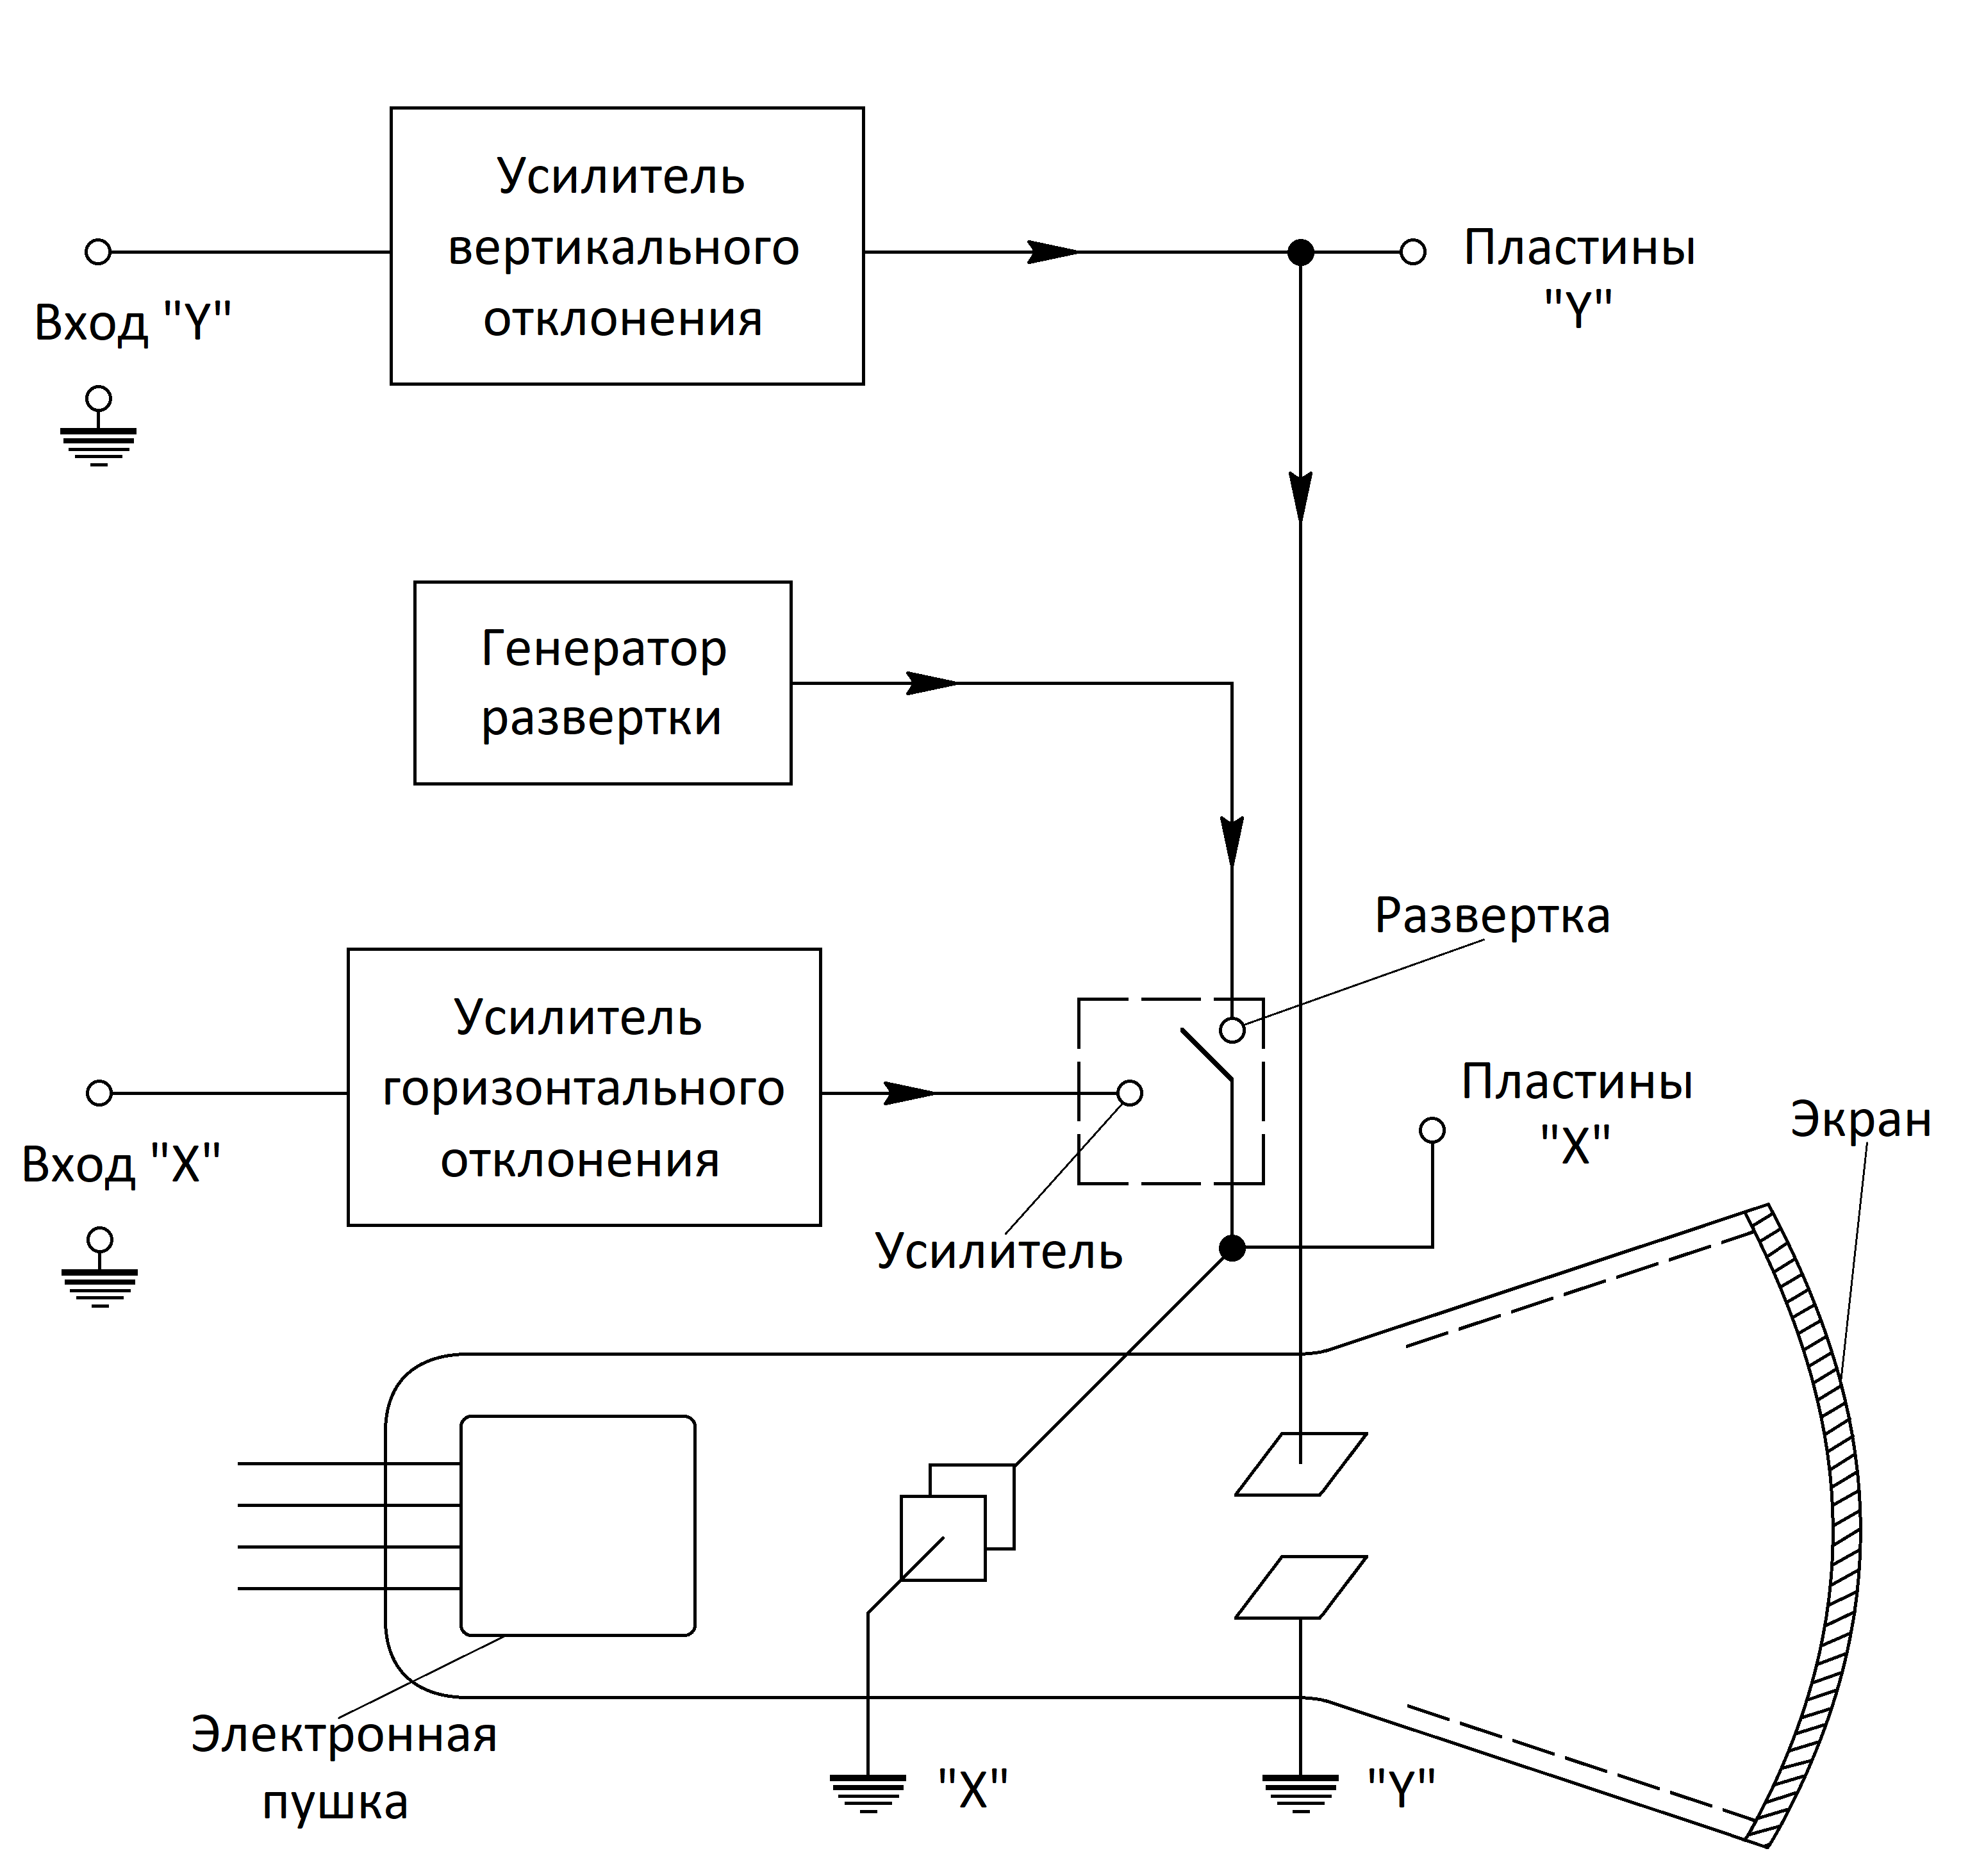
\includegraphics[width=0.9\textwidth]{Scheme2.png}
\caption{Упрощенная блок-схема осциллографа}
\label{fig:Scheme2}
\end{figure}

\subsection{Эксперимент}
На рис.~\ref{fig:Photo1} представлена фотография электронного осциллографа (С1-19Б), на рис.~\ref{fig:Photo2} фотография генератора синусоидального напряжения (Г3-109) и испытательного стенда, состоящего из двух плат: для исследования чувствительности пластин и наблюдения фигур Лиссажу и для исследования чувствительности осциллографа. В ходе работы были собраны две цепи с использованием обеих плат поочередно, измерены чувствительности обеих пластин для различных длин отображаемой на экране линии и максимальная чувствительность осциллографа, получены фигуры Лиссажу.

\begin{figure}[H]
\centering
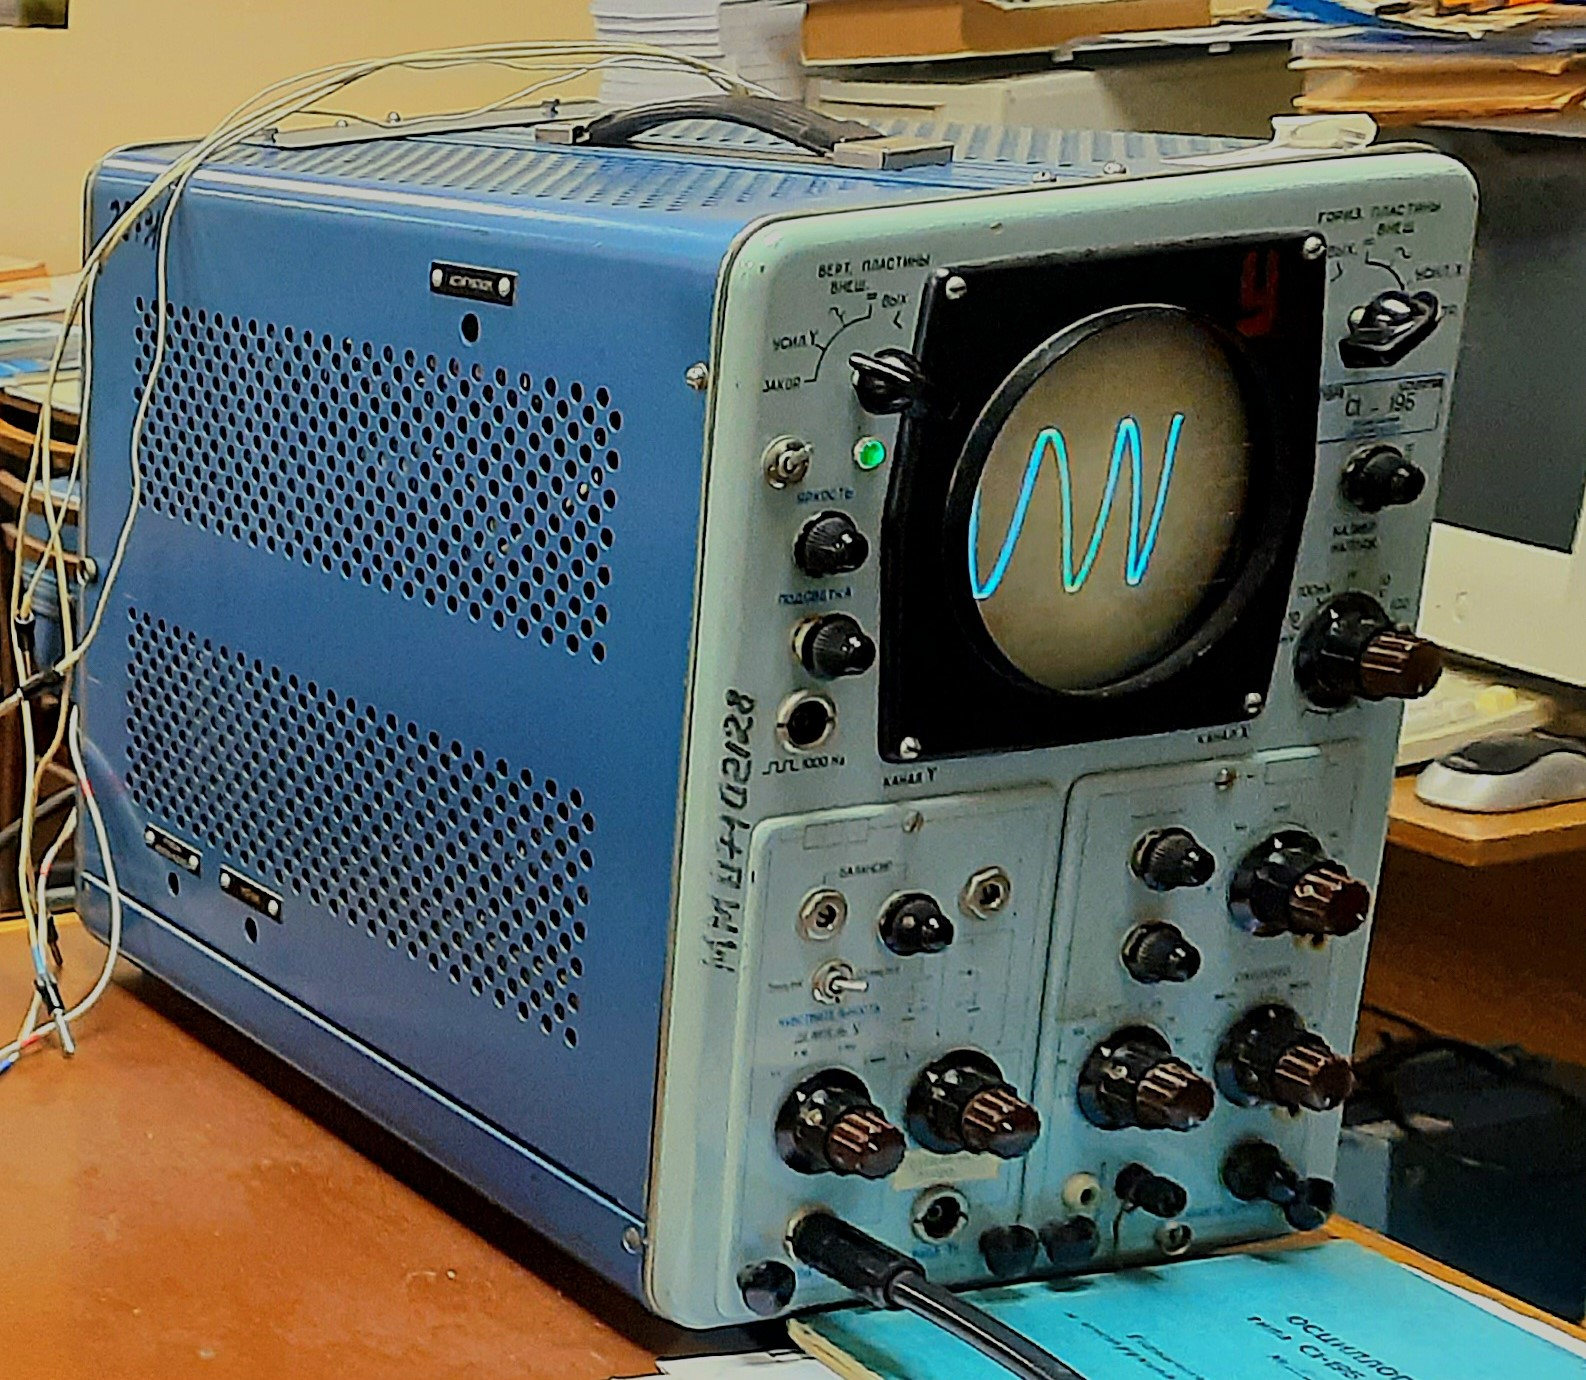
\includegraphics[width=0.8\textwidth]{Photo1.jpg}
\caption{Фотография электронного осциллографа (С1-19Б)}
\label{fig:Photo1}
\end{figure}

\begin{figure}[H]
\centering
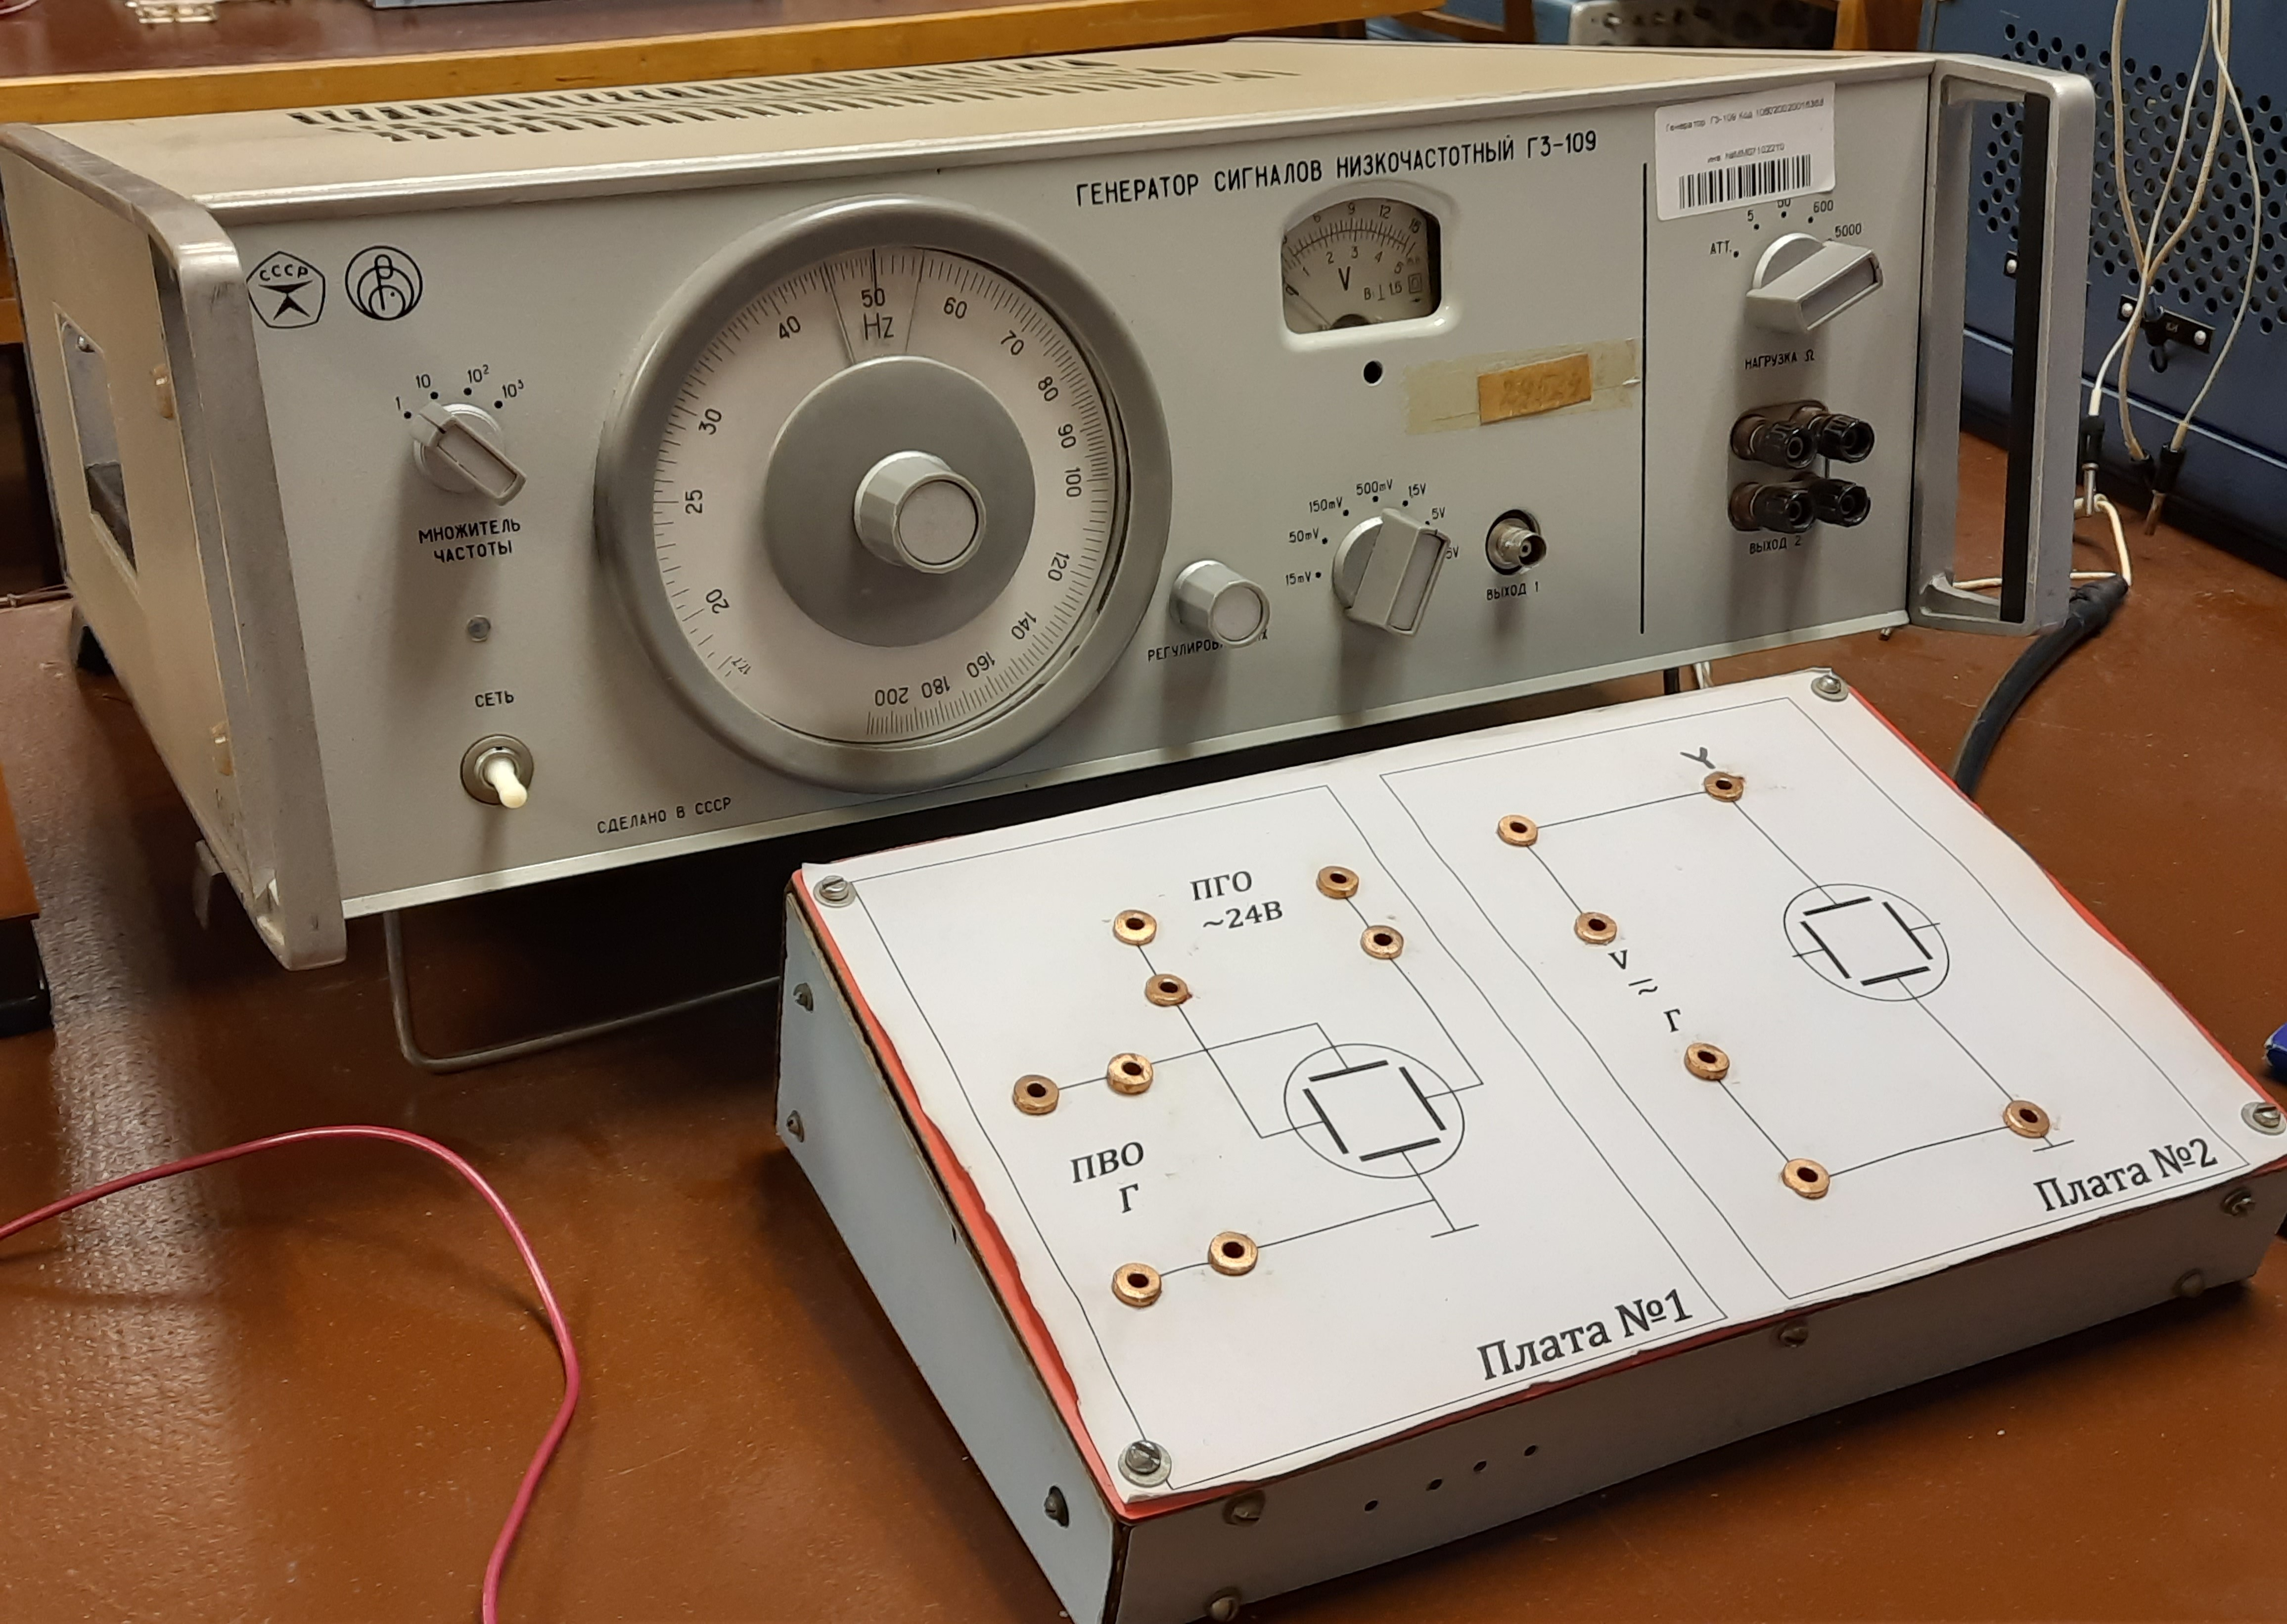
\includegraphics[width=0.8\textwidth]{Photo2.jpg}
\caption{Фотография генератора синусоидального напряжения (Г3-109) и испытательного стенда (плат №1 и №2)}
\label{fig:Photo2}
\end{figure}

На рис.~\ref{fig:Scheme3} и рис.~\ref{fig:Scheme4} представлены схемы электрических цепей для исследования чувствительности пластин испытательного стенда и получения фигур Лиссажу, и для наблюдения исследуемого напряжения и определения максимальной чувствительности осциллографа.

\begin{figure}[H]
\centering
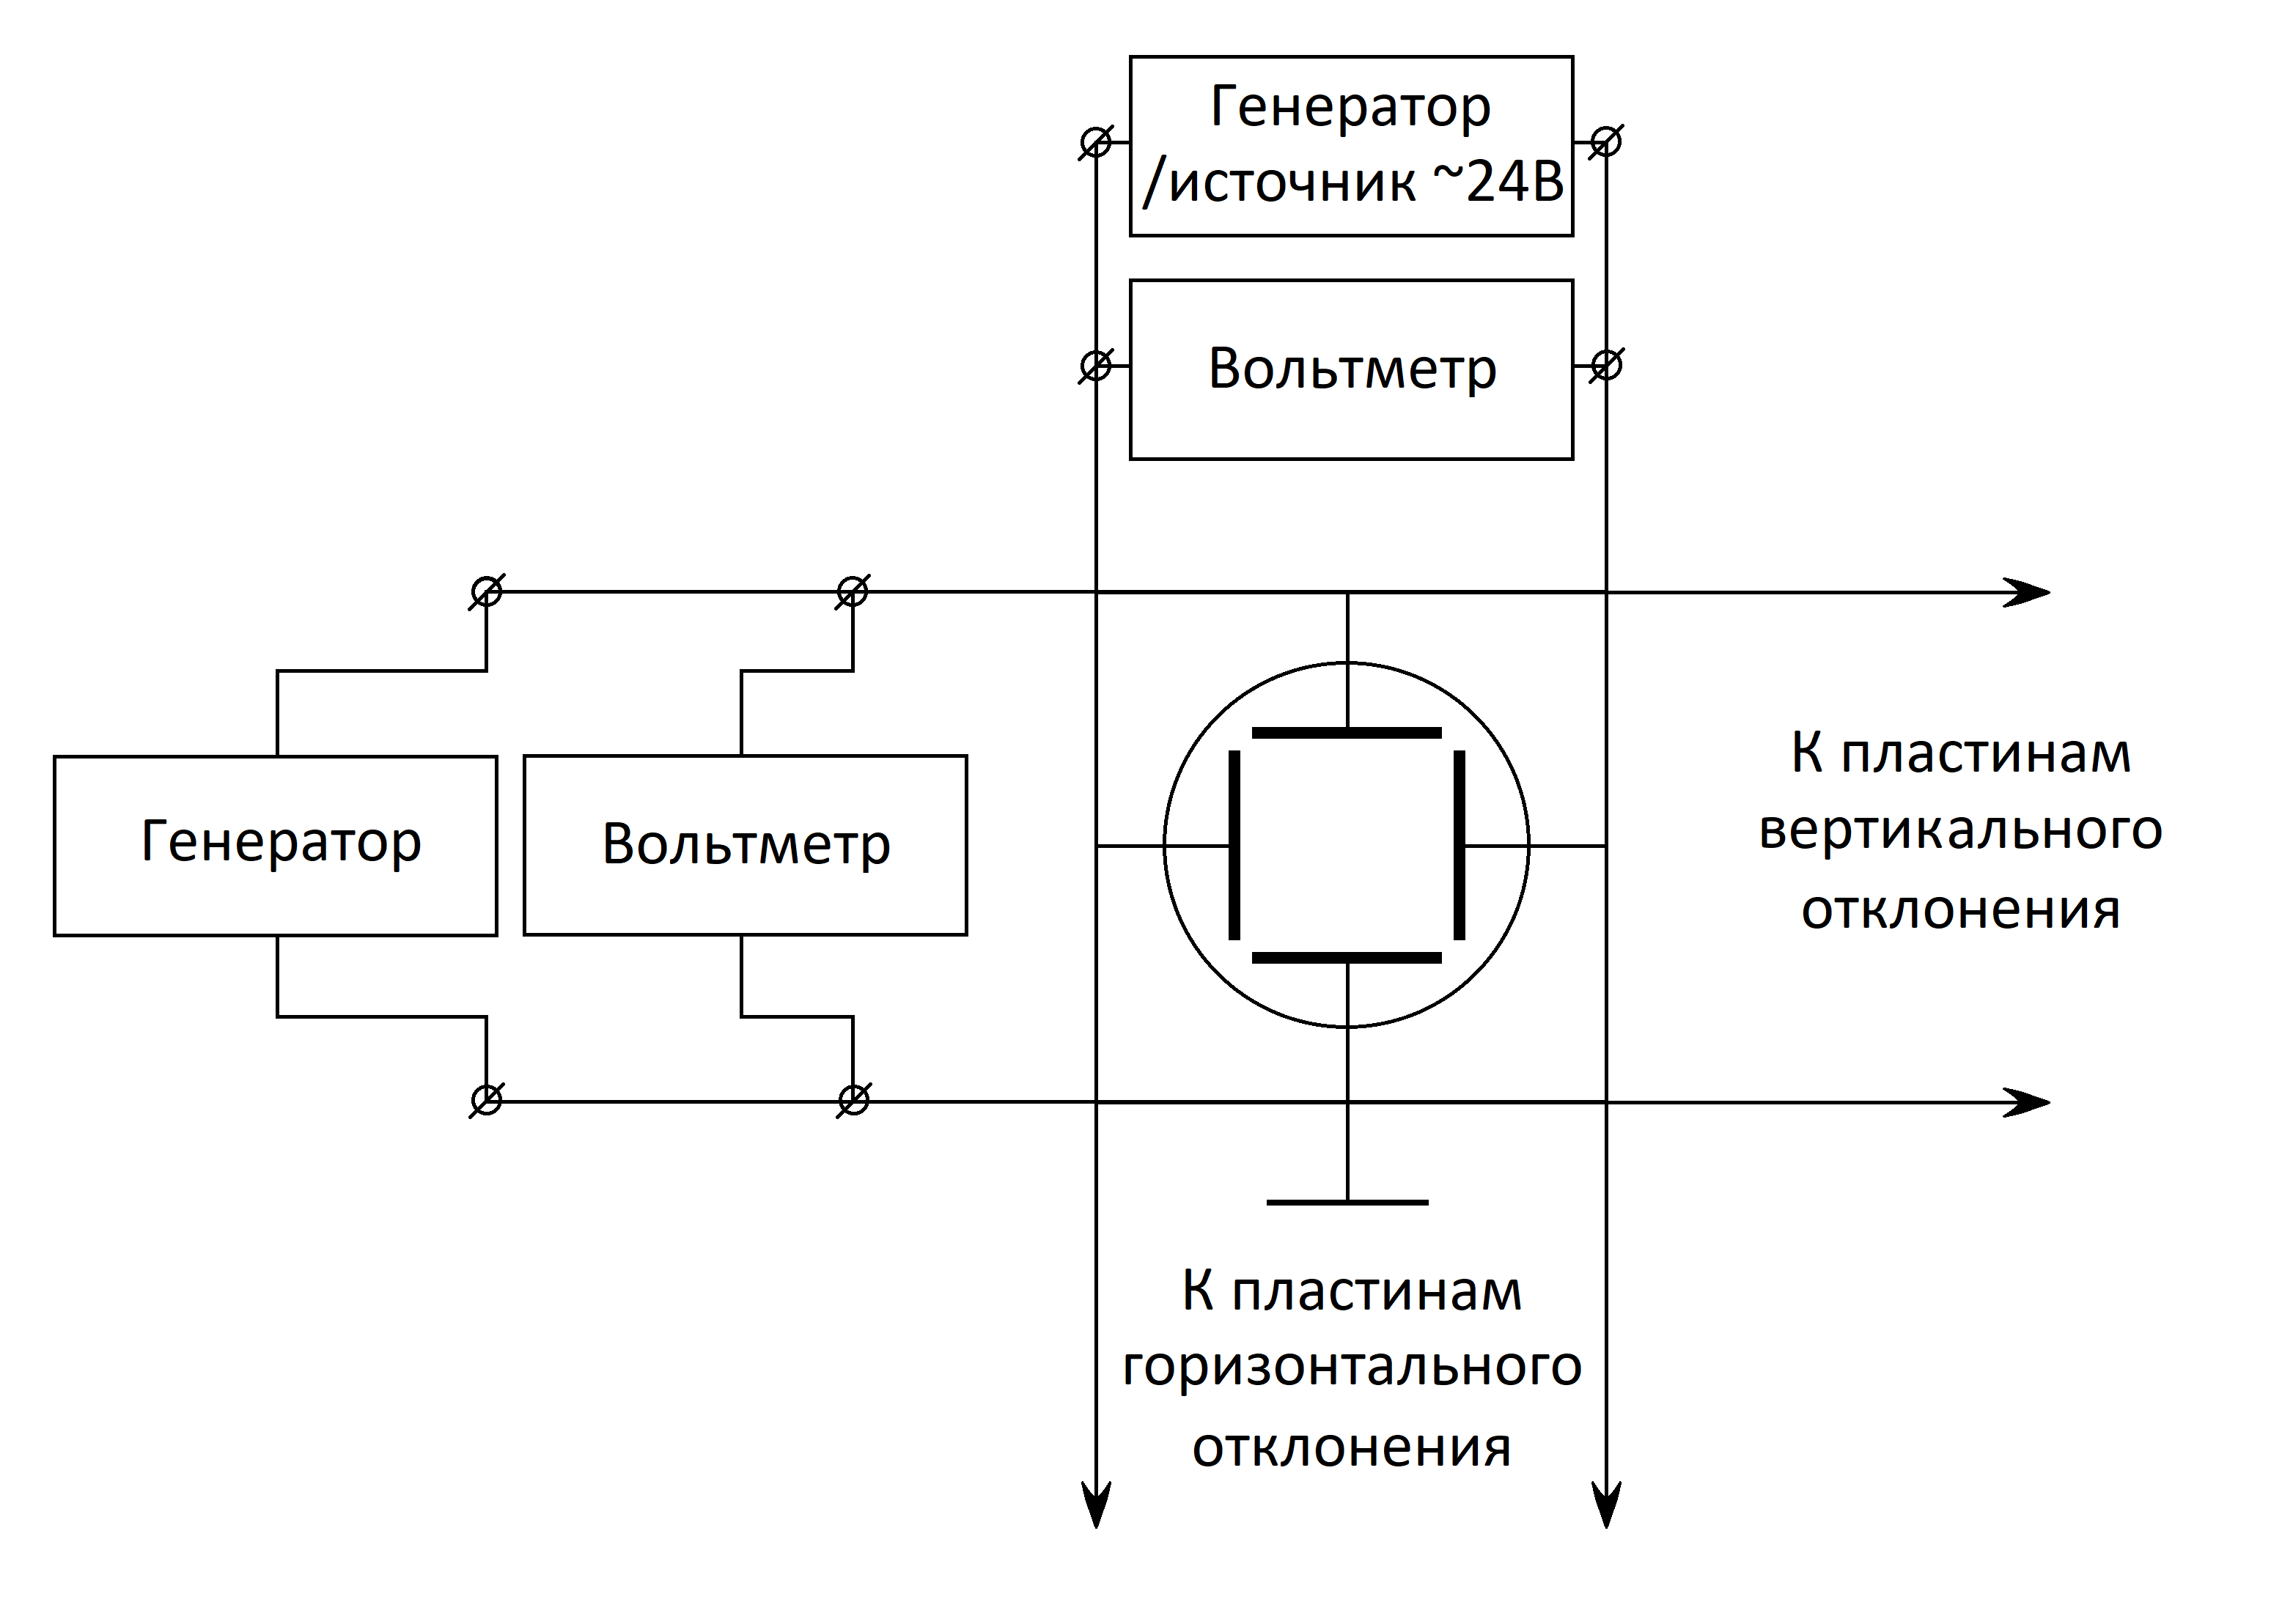
\includegraphics[width=0.8\textwidth]{Scheme3.png}
\caption{Схема электрической цепи для исследования чувствительности пластин электронно-лучевой трубки и получения фигур Лиссажу}
\label{fig:Scheme3}
\end{figure}

\begin{figure}[H]
\centering
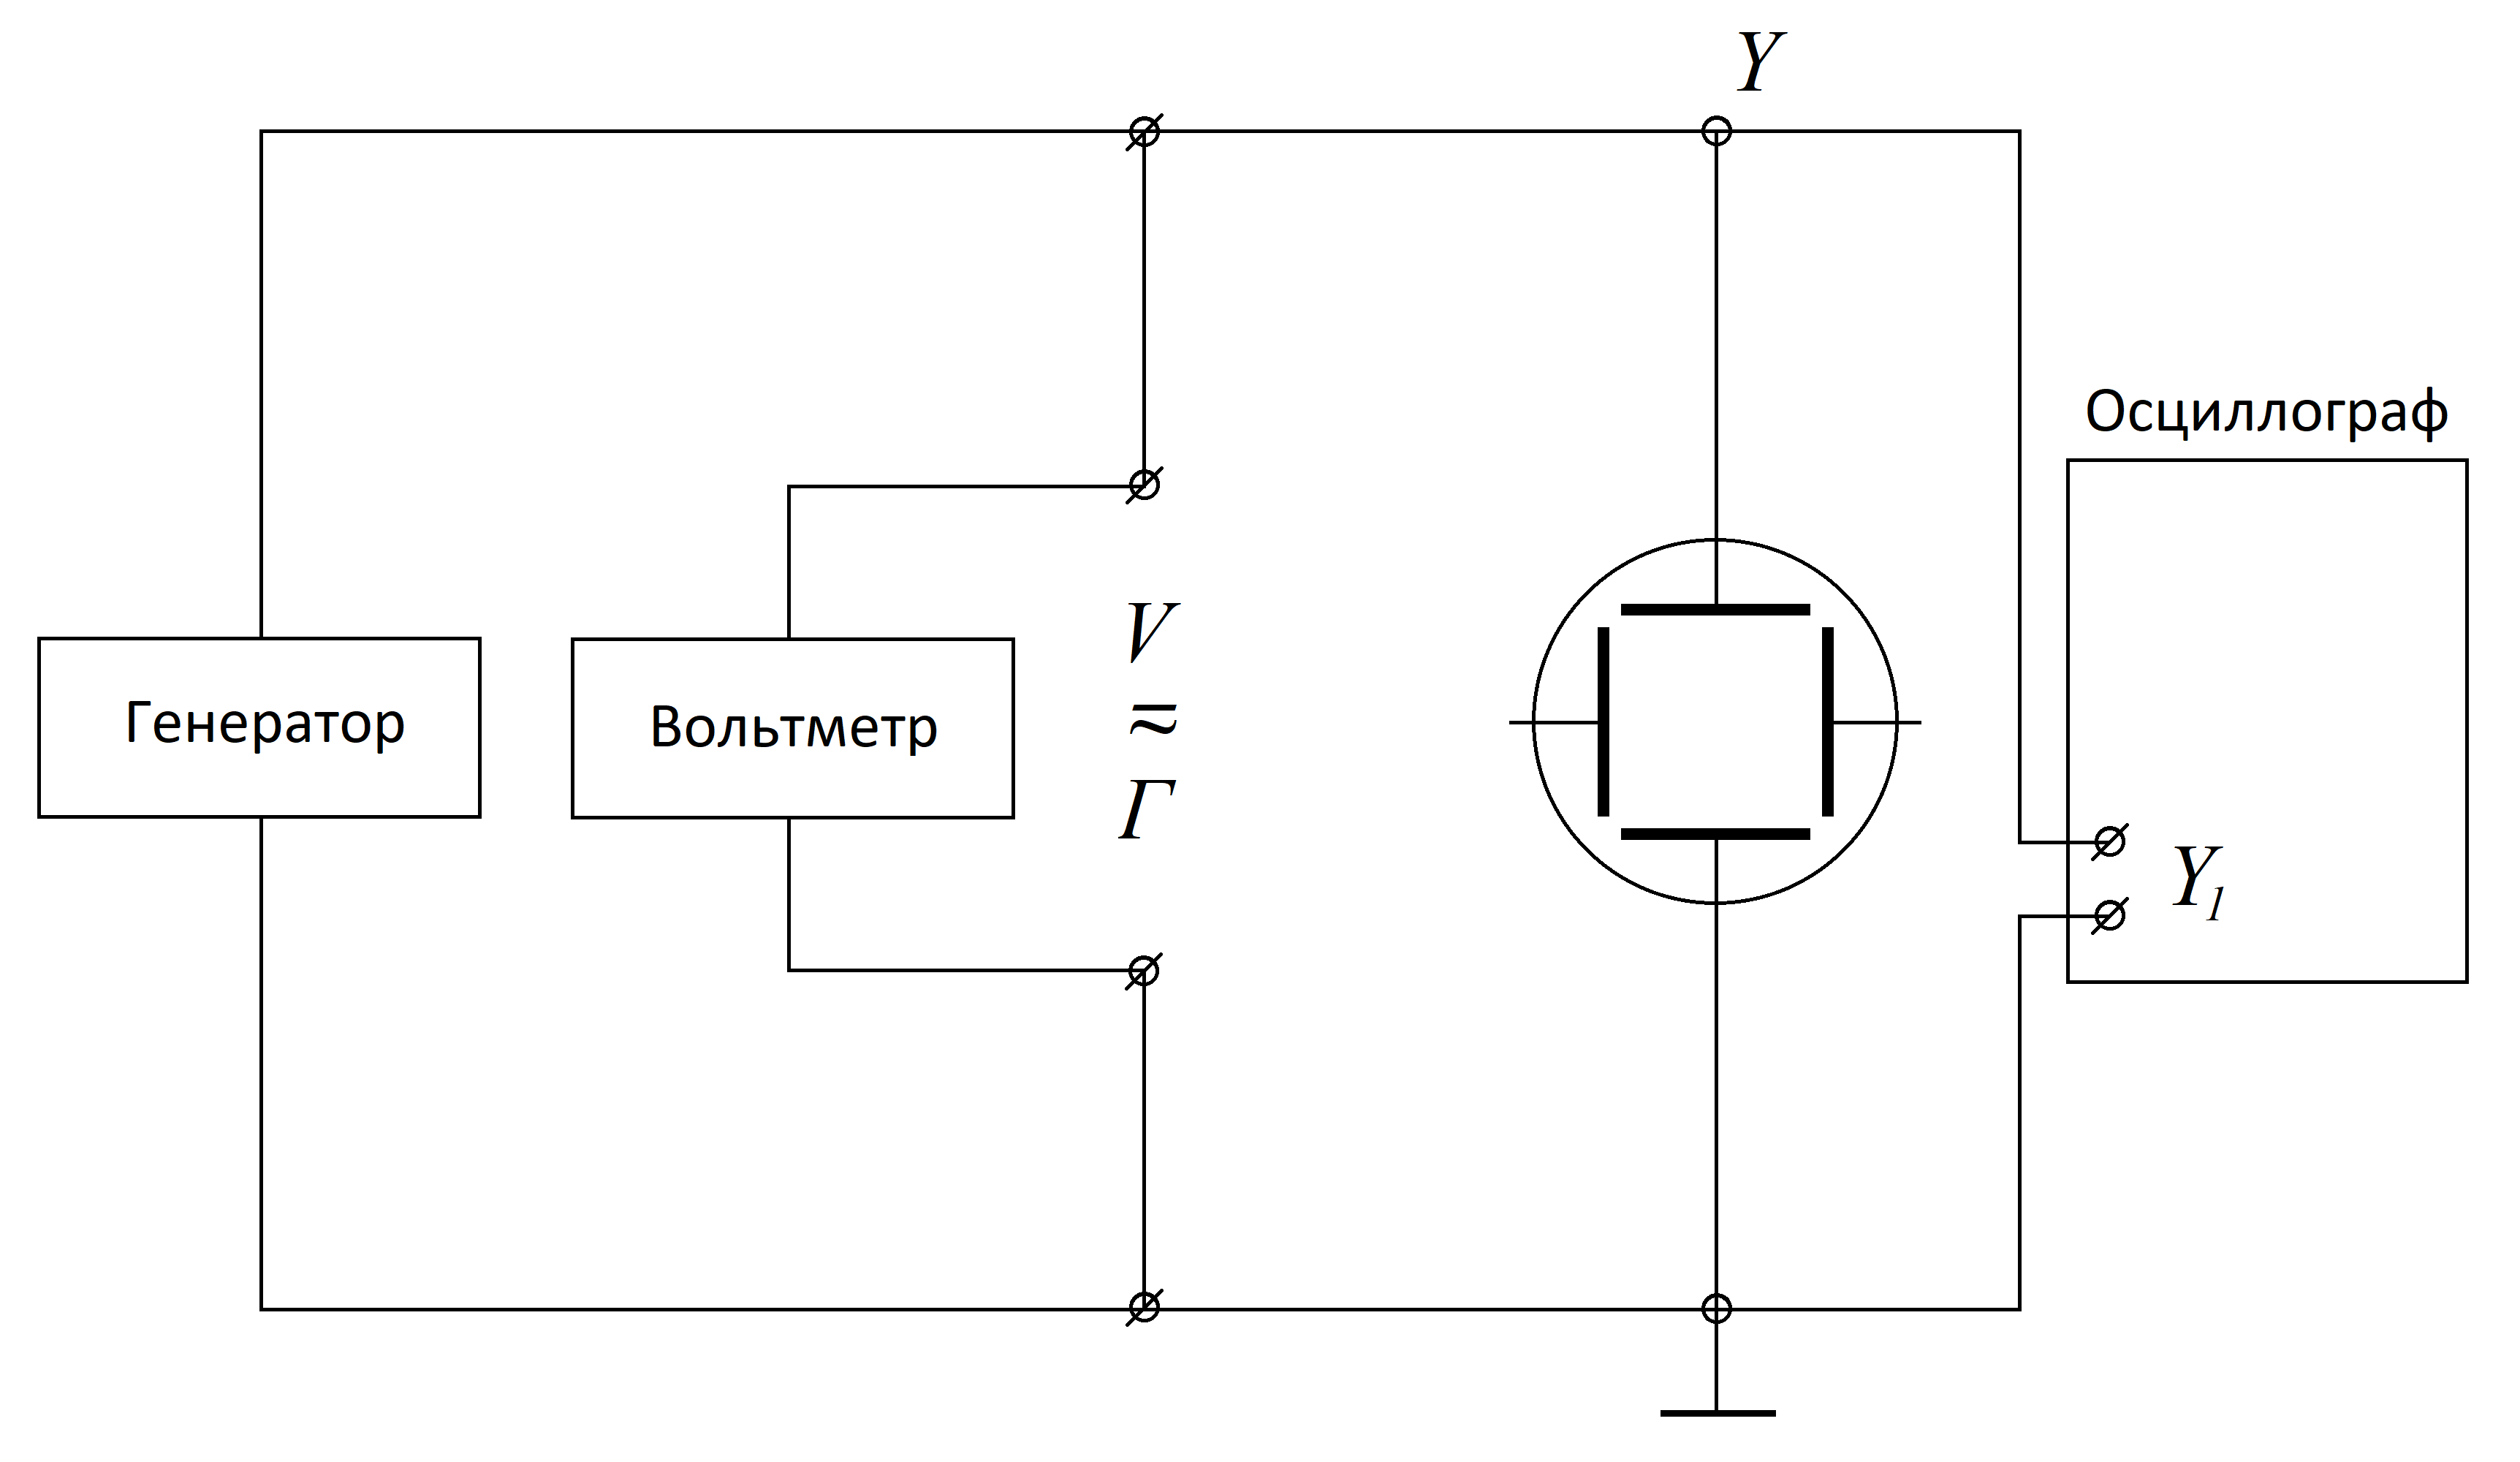
\includegraphics[width=0.8\textwidth]{Scheme4.png}
\caption{Схема электрической цепи для наблюдения исследуемого напряжения и определения максимальной чувствительности осциллографа}
\label{fig:Scheme4}
\end{figure}

\subsection{Обработка данных и обсуждение результатов}
 
\subsubsection{Таблицы}

\begin{center}
\begin{table}[H]
\centering
\caption{Пластины вертикального отклонения (ПВО)}
\label{tabl:1}
\renewcommand{\arraystretch}{1.15}
\begin{tabular}{|c|c|c|c|}
\hline
\begin{minipage}{5cm}
\begin{center}
    Длина линии на экране, L
\end{center}
\end{minipage} &
\begin{minipage}{5cm}
\begin{center}
    Эффективное напряжение, $U_{\text{eff}}$
\end{center}
\end{minipage} &
\begin{minipage}{5cm}
\begin{center}
    Чувствительность, S
\end{center}
\end{minipage}\\
\hline
мм&В&мм/В\\
\hline
10  &  5.50  &  0.64 \\
20  &  11.5  &  0.62 \\
30  &  18.1  &  0.59 \\
40  &  24.5  &  0.58 \\
50  &  31.5  &  0.56 \\
\hline
\end{tabular}
\end{table}
\end{center}

Для чувствительности пластин вертикального отклонения на основе полученных в ходе эксперимента данных, приведенных в таблице ~\ref{tabl:1}, при которых $S_y$ слабо зависит от $U_{\text{eff}}$ (при длине L равной 20, 30 и 40 мм), было высчитано среднее значение $\overline{S_y} = 0.60$ мм/В и вычислена погрешность результата прямых измерений по общепринятым правилам по отклонению от среднего по формуле:

\begin{equation}
\label{eq:5}
   \Delta S=\sqrt{\frac{\Sigma{(S_i-\overline{S})^2}}{n(n-1)}}
\end{equation}

Таким образом, $\Delta S_y = 0.12$ мм/В.

\begin{center}
\begin{table}[H]
\centering
\caption{Пластины горизонтального отклонения (ПГО)}
\label{tabl:2}
\renewcommand{\arraystretch}{1.15}
\begin{tabular}{|c|c|c|c|}
\hline
\begin{minipage}{5cm}
\begin{center}
    Длина линии на экране, L
\end{center}
\end{minipage} &
\begin{minipage}{5cm}
\begin{center}
    Эффективное напряжение, $U_{\text{eff}}$
\end{center}
\end{minipage} &
\begin{minipage}{5cm}
\begin{center}
    Чувствительность, S
\end{center}
\end{minipage}\\
\hline
мм&В&мм/В\\
\hline
10  &  4.70  &  0.75 \\
20  &  11.1  &  0.64 \\
30  &  17.1  &  0.62 \\
40  &  24.1  &  0.59 \\
50  &  29.3  &  0.60 \\
\hline
\end{tabular}
\end{table}
\end{center}

Для чувствительности пластин горизонтального отклонения на основе полученных в ходе эксперимента данных, приведенных в таблице ~\ref{tabl:2}, при которых $S_x$ слабо зависит от $U_{\text{eff}}$ (при длине L равной 20, 30 и 40 мм), было высчитано среднее значение $\overline{S_x} = 0.62$ мм/В и вычислена погрешность результата прямых измерений по формуле (~\ref{eq:5}), $\Delta S_x = 0.015$ мм/В.

\begin{center}
\begin{table}[H]
\centering
\caption{Максимальная чувствительность осциллографа}
\label{tabl:3}
\renewcommand{\arraystretch}{1.15}
\begin{tabular}{|c|c|c|c|}
\hline
\begin{minipage}{5cm}
\begin{center}
    Длина линии на экране, L
\end{center}
\end{minipage} &
\begin{minipage}{5cm}
\begin{center}
    Эффективное напряжение, $U_{\text{eff}}$
\end{center}
\end{minipage} &
\begin{minipage}{5cm}
\begin{center}
    Чувствительность, S
\end{center}
\end{minipage}\\
\hline
мм&В&мм/В\\
\hline
10  &  0.010  &  $35\cdot10$ \\
20  &  0.023  &  $31\cdot10$ \\
30  &  0.037  &  $29\cdot10$ \\
40  &  0.052  &  $27\cdot10$ \\
50  &  0.064  &  $28\cdot10$ \\
\hline
\end{tabular}
\end{table}
\end{center}

Максимальная чувствительность осциллографа вычисляется по следующей формуле:

\begin{equation}
\label{eq:6}
   (S'_y)_m=\frac{L'}{2\sqrt{2}U'_\text{{eff}}}
\end{equation}

где $L'$ — двойная амплитуда синусоиды, проявляющейся на экране осциллографа в мм, а $U'_\text{{eff}}$ — напряжение, подаваемое на вход осциллографа в В.

Было высчитано среднее значение максимальной чувствительности осциллографа: $\overline{(S'_y)_m} = 30\cdot10$ мм/В.

Максимальный коэффициент усиления осциллографического усилителя вычисляется по формуле:

\begin{equation}
\label{eq:7}
   K_m=\frac{(\overline{S'_y)_m}}{\overline{S_y}}
\end{equation}

Таким образом, $K_m=50\cdot10$.

\begin{center}
\begin{table}[H]
\centering
\caption{Измерение неизвестной частоты при наблюдении фигур Лиссажу}
\label{tabl:4}
\renewcommand{\arraystretch}{1.5}
\begin{tabular}{|c|c|c|c|c|}
\hline
\begin{minipage}{8cm}
\begin{center}
    Вид фигуры Лиссажу
\end{center}
\end{minipage} &
\begin{minipage}{2cm}
\begin{center}
    
\begin{tikzpicture}[scale=0.5]
      \draw[blue, thick] 
      plot [domain=0:360, samples=300] ({sin(\x)}, {cos(\x)});
    \end{tikzpicture}
\end{center}
\end{minipage} &
\begin{minipage}{2cm}
\begin{center}
    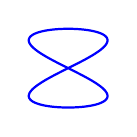
\begin{tikzpicture}[scale=0.5]
      \draw[blue, thick] 
      plot [domain=0:360, samples=300] ({sin(2*\x)}, {cos(\x)});
    \end{tikzpicture}
\end{center}
\end{minipage} &
\begin{minipage}{2cm}
\begin{center}
    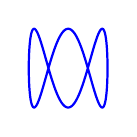
\begin{tikzpicture}[scale=0.5]
      \draw[blue, thick] 
      plot [domain=0:360, samples=300] ({cos(\x)}, {sin(3*\x)});
    \end{tikzpicture}
\end{center}
\end{minipage} &
\begin{minipage}{2cm}
\begin{center}
    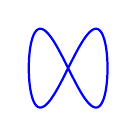
\begin{tikzpicture}[scale=0.5]
      \draw[blue, thick] 
      plot [domain=0:360, samples=300] ({cos(\x)}, {sin(2*\x)});
    \end{tikzpicture}
\end{center}
\end{minipage}\\
\hline
Отношение частот  $f_x : f_y$ &  1:1 &  2:1 & 1:3 & 1:2 \\
Частота по лимбу генератора, $f_y$, Гц &  $50\pm{}0.5$  & $25\pm{}0.5$ & $150\pm{}0.5$ & $100\pm{}0.5$\\
Исследуемая частота, $f_x$, Гц  &  $50\pm{}0.5$  &  $50\pm{}0.5$ & $50\pm{}0.5$ & $50\pm{}0.5$ \\
\hline
\end{tabular}
\end{table}
\end{center}

\subsubsection{Описание программ}

Для проведения расчётов на языке C++ были написаны программы ``Sx'', ``Sy'' и ``max S'', предназначенные для обработки данных, связанных с чувствительностью пластин горизонтального и вертикального отклонений электронно-лучевой трубки осциллографа, а также для вычисления максимальной чувствительности осциллографа и коэффициента усиления.

Программа ``Sx'' состоит из следующих функций:
\begin{itemize}
\item in(): отвечает за ввод данных из файла ``Input.csv'' в двумерный массив a, где каждая строка содержит длину линии на экране (в мм) и эффективное напряжение (в В).
\item roundx(): округляет число до указанного количества значащих цифр.
\item colSi(): вычисляет значения чувствительности пластин горизонтального отклонения $S_x$ для каждой строки данных по формуле (\ref{eq:2}).
\item Sx(): вычисляет среднее значение чувствительности $S_x$ для данных строк (исключая первую и последнюю строки).
\item dSx(): вычисляет погрешность среднего значения $S_x$ по формуле стандартного отклонения от среднего (\ref{eq:5}).
\item out(): записывает в файл ``Output.csv'' значения $S_x$ для каждой строки, среднее значение $S_x$ и его погрешность.
\end{itemize}

Программа ``Sy'' имеет аналогичную структуру и в точности совпадающие функции, но предназначена для расчёта чувствительности пластин вертикального отклонения $S_y$.

Программа ``max S'' предназначена для вычисления максимальной чувствительности осциллографа и коэффициента усиления усилителя. Она включает следующие функции:

\begin{itemize}
\item in(): отвечает за ввод данных из файла ``Input.csv''.
\item roundx(): округляет число до указанного количества значащих цифр.
\item colSi(): вычисляет значения максимальной чувствительности $S_{max}$ для каждой строки данных по формуле (\ref{eq:2}).
\item avrgS(): вычисляет среднее значение $S_{max}$.
\item Km(): вычисляет коэффициент усиления усилителя по формуле (\ref{eq:7}).
\item out(): записывает в файл ``Output.csv'' значения $S_{max}$ для каждой строки, среднее значение $S_{max}$ и коэффициент усиления $K_m$.
\end{itemize}

\subsubsection{Графики}

На рис.~\ref{fig:plot1}, рис.~\ref{fig:plot2} приведены результаты работы программы gnuplot для графиков зависимости $S_y = f(U_{\text{eff}})$ и $S_x = f(U_{\text{eff}})$ соответственно.

\begin{figure}[H]
\centering
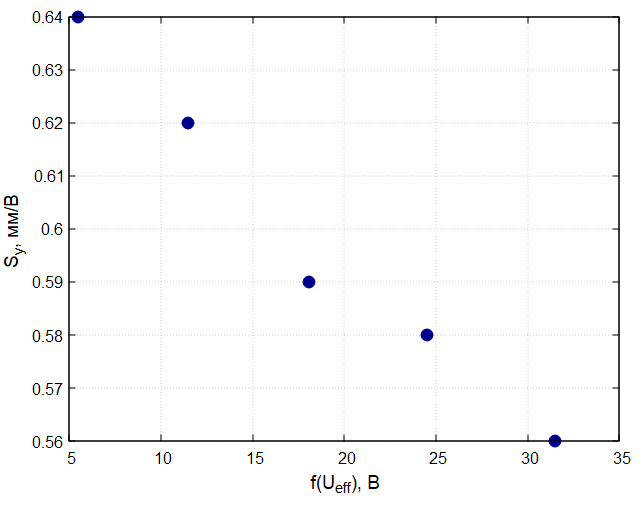
\includegraphics[width=0.8\textwidth]{plot1.png}
\caption{График зависимости $S_y = f(U_{\text{eff}})$}
\label{fig:plot1}
\end{figure}

\begin{figure}[H]
\centering
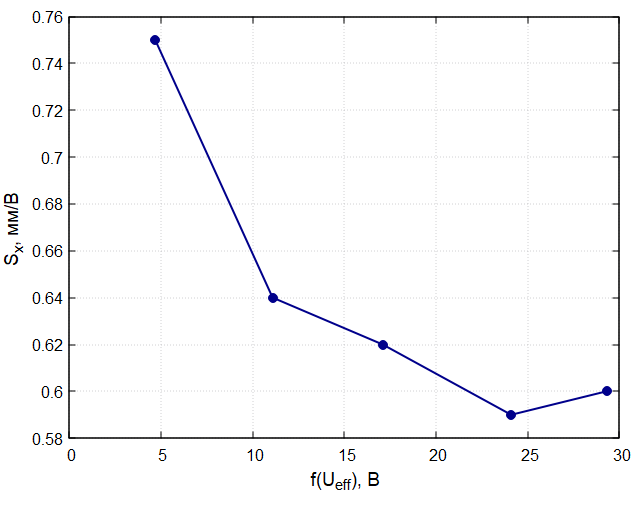
\includegraphics[width=0.8\textwidth]{plot2.png}
\caption{График зависимости $S_x = f(U_{\text{eff}})$}
\label{fig:plot2}
\end{figure}

\section{Вывод}

В ходе лабораторной работы было проведено исследование характеристик электронного осциллографа, включая определение чувствительности пластин вертикального и горизонтального отклонения, а также изучение фигур Лиссажу. Определены средние значения чувствительности вертикальных и горизонтальных пластин, установлены максимальная чувствительность прибора и коэффициент усиления. Исследование фигур Лиссажу продемонстрировало возможности осциллографа в анализе и визуализации сложных сигналов. Результаты работы показали, что осциллограф является эффективным инструментом для визуализации и анализа электрических сигналов, а также определения их параметров с высокой точностью.

\begin{thebibliography}{9}
\bibitem{repo}
\url{https://github.com/st117208/Workshop3}  (дата обращения: 11.04.2025)
\end{thebibliography}